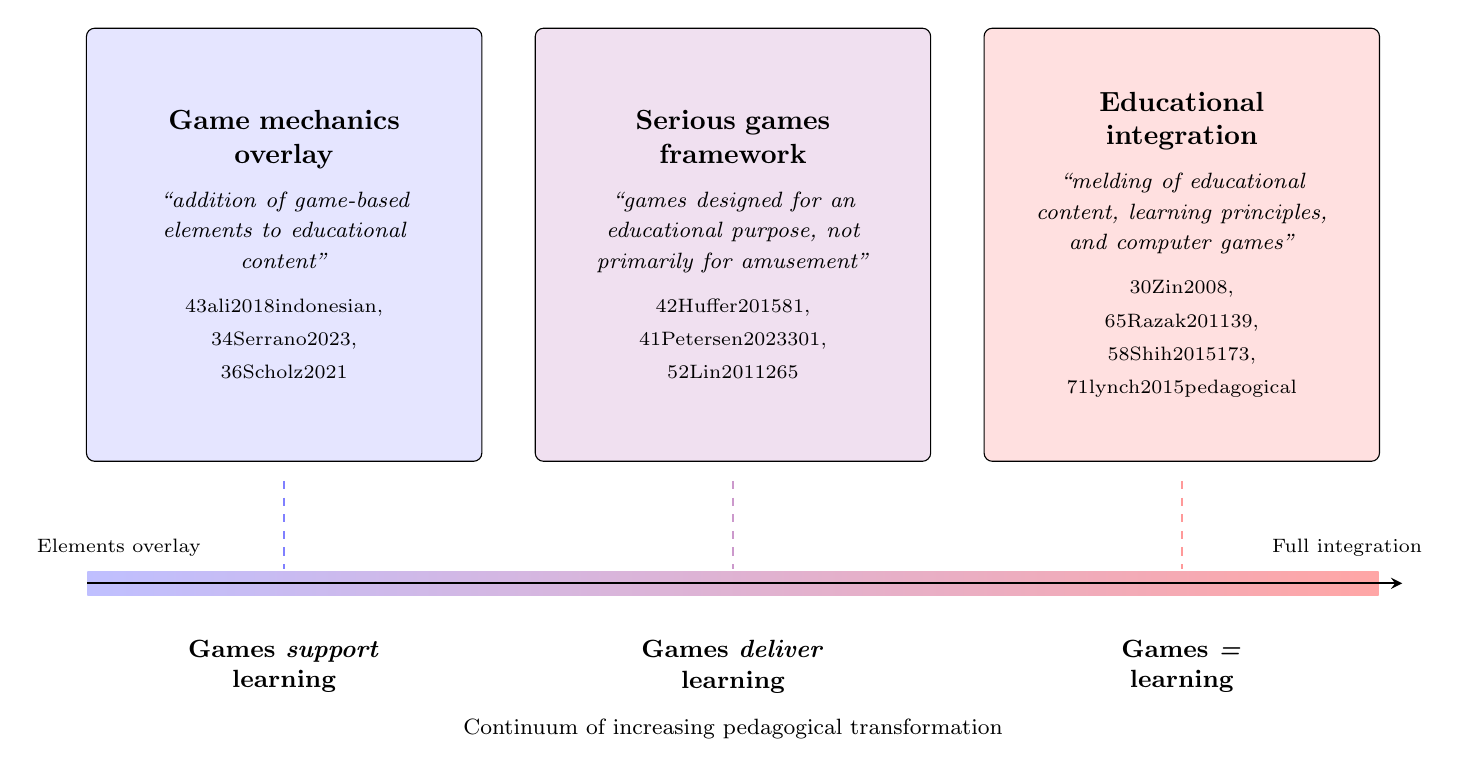
\begin{tikzpicture}
\tikzstyle{framebox} = [rectangle, draw, rounded corners=3pt,
  minimum width=5.0cm, minimum height=5.5cm, text width=4.6cm, align=center, inner sep=6pt]
\tikzstyle{relabel} = [font=\small\bfseries, anchor=north, align=center]

% Framing 1
\node[framebox, fill=blue!10] (F1) at (2.8, 3.8) {%
  \textbf{Game mechanics}\\
  \textbf{overlay}\\[4pt]
  {\footnotesize\itshape ``addition of game-based}\\[-1pt]
  {\footnotesize\itshape elements to educational}\\[-1pt]
  {\footnotesize\itshape content''}\\[4pt]
  {\scriptsize \mbox{\citet{43ali2018indonesian}},}\\
  {\scriptsize \mbox{\citet{34Serrano2023}},}\\
  {\scriptsize \mbox{\citet{36Scholz2021}}}%
};

% Framing 2
\node[framebox, fill=violet!12] (F2) at (8.5, 3.8) {%
  \textbf{Serious games}\\
  \textbf{framework}\\[4pt]
  {\footnotesize\itshape ``games designed for an}\\[-1pt]
  {\footnotesize\itshape educational purpose, not}\\[-1pt]
  {\footnotesize\itshape primarily for amusement''}\\[4pt]
  {\scriptsize \mbox{\citet{42Huffer201581}},}\\
  {\scriptsize \mbox{\citet{41Petersen2023301}},}\\
  {\scriptsize \mbox{\citet{52Lin2011265}}}%
};

% Framing 3
\node[framebox, fill=red!12] (F3) at (14.2, 3.8) {%
  \textbf{Educational}\\
  \textbf{integration}\\[4pt]
  {\footnotesize\itshape ``melding of educational}\\[-1pt]
  {\footnotesize\itshape content, learning principles,}\\[-1pt]
  {\footnotesize\itshape and computer games''}\\[4pt]
  {\scriptsize \mbox{\citet{30Zin2008}},}\\
  {\scriptsize \mbox{\citet{65Razak201139}},}\\
  {\scriptsize \mbox{\citet{58Shih2015173}},}\\
  {\scriptsize \mbox{\citet{71lynch2015pedagogical}}}%
};

% Connector lines
\draw[thick, blue!50, dashed] (2.8, 0.8) -- (2.8, -0.32);
\draw[thick, violet!40, dashed] (8.5, 0.8) -- (8.5, -0.32);
\draw[thick, red!40, dashed] (14.2, 0.8) -- (14.2, -0.32);

% Gradient arrow bar
\shade[left color=blue!25, right color=red!35] (0.3,-0.65) rectangle (16.7,-0.35);
\draw[thick, ->, >=stealth] (0.3,-0.5) -- (17.0,-0.5);

% Endpoint labels
\node[font=\scriptsize, anchor=south] at (0.7, -0.28) {Elements overlay};
\node[font=\scriptsize, anchor=south] at (16.3, -0.28) {Full integration};

% Relationship descriptors below
\node[relabel] at (2.8, -1.1) {Games \textit{support}\\learning};
\node[relabel] at (8.5, -1.1) {Games \textit{deliver}\\learning};
\node[relabel] at (14.2, -1.1) {Games \textit{=}\\learning};

% Bottom label
\node[font=\footnotesize, anchor=north] at (8.5, -2.1)
  {Continuum of increasing pedagogical transformation};

\end{tikzpicture}
